\subsection{Global Hypothesis Test}
\datum{Lecture 2: 01/08}
\begin{defn}[valid p-value]
    Given null-hypotheses $H_{0, 1}, \dots, H_{0,m}$ with p-values $p_1, \dots, p_m$. Then $p_i$ is \emph{valid} if $\mathbb{P}\{p_i \leq \alpha\}$ holds for all $\alpha \in [0,1]$, i.e. it is \textit{superuniform}. 
\end{defn}

\begin{defn}[Stochastic Ordering]
    $X \stackrel{\text{St}}{<} Y$ \, iff \, $\mathbb{P}\{X\leq t\} \geq \mathbb{P}\{Y\geq t\}$ for all $t\in \mathbb{R}$.
\end{defn}


\begin{proposition}[Bonferroni Test]
    The \emph{Bonferroni test} rejects $H_{0,\textup{global}}$ if $\min_{i=1,\dots,m} p_i \leq \frac{\alpha}{m}$.
\end{proposition}
\begin{pr}
\begin{align*}
    \mathbb{P}\{\textup{Bonferroni rejects } H_{0, \text{global}}\} &= \mathbb{P}_{H_{0, \text{global}}}\{\min_i p_i \leq \frac{\alpha}{m}\} \\
    &\leq \sum_{i=1}^m \mathbb{P}_{H_{0, \text{global}}}\{p_i \leq \frac{\alpha}{m}\} \\
    &= m\cdot\frac{\alpha}{m} = \alpha.
    \end{align*}
\end{pr}

\begin{proposition}[Fisher Test]
    The \emph{Fisher test} rejects $H_{0,\textup{global}}$ if $-2 \sum_{i=1}^m \log(p_i) \geq F^{-1}_{\chi_{2m}^2}(1-\alpha)$.
\end{proposition}

\emph{\textbf{Fact.}} If $U \sim \textup{Uniform}[0,1]$, then $-2\log(U) \sim \chi^2_2$ $\implies$ If $p_1, \dots, p_m  \sim \textup{Uniform}[0,1]$ and independent, then $-2\sum_{i=1}^m\log(p_i) \sim \chi^2_{2m}$ $\implies$ If $p_1,\dots, p_m$ are super-uniform under nulls and independent, then $-2\sum_{i=1}^m \log(p_i) \sim \chi^2_{2m}$.

\emph{\textbf{Extreme Case.}} If correlation between $p_1,\dots,p_m$ is 1 for all pairs, then $-2 \sum_{i=1}^m \log(p_i) = m \log(p_i) = m\chi^2_2$ with variance $O(m^2)$ compared to $O(m)$ of $\chi^2_{2m}$. Thus correlated p-values can easily yield an inflated Fisher test.

Use Fisher test if $p$-values are expected to be independent, otherwise use Bonferroni test. However, this would give us two chances to reject the null and in the worst case the significance level becomes $2\alpha$ (Bonferroni inequality) instead of $\alpha$. One solution would be to run both tests with a significance level of $\frac{\alpha}{2}$. Another test that accounts for this is the Simes test.

\begin{proposition}{Simes Test}
    The \emph{Simes test} rejects $H_{0,\textup{global}}$ if for any $k = 1,\dots,m$, there are more than $k$ values of $p_i$ with $p_i \leq \frac{\alpha k}{m}$.    
\end{proposition}


By considering $k=1$, we can see that if the Bonferroni test rejects $H_0$, so does the Fisher test.
\newpage
\begin{figure}[h!]
    \centering
    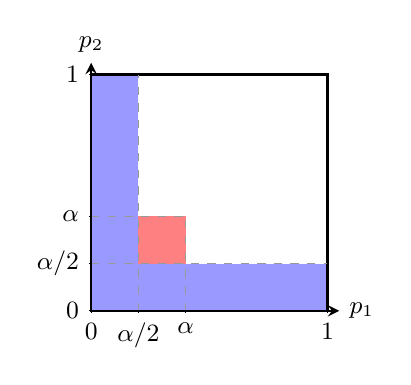
\begin{tikzpicture}[scale=0.3, >=stealth, font=\small]
    % Define coordinates for cleaner code based on arbitrary units
    % Scale: 10 units = 1.
    % Therefore: 2 units = alpha/2, 4 units = alpha.
    \coordinate (O) at (0,0);
    \coordinate (XEnd) at (10.5,0);
    \coordinate (YEnd) at (0,10.5);
    \coordinate (A2_x) at (2,0); % alpha/2 on x
    \coordinate (A_x) at (4,0);  % alpha on x
    \coordinate (One_x) at (10,0); % 1 on x
    \coordinate (A2_y) at (0,2); % alpha/2 on y
    \coordinate (A_y) at (0,4);  % alpha on y
    \coordinate (One_y) at (0,10); % 1 on y

    % --- SHADING REGIONS ---

    % Region 1: Bonferroni Rejection Region (also Simes Rejection)
    % Rule: Reject if ANY p_i <= alpha/m (here alpha/2)
    \fill[blue!40] (O) rectangle (One_x |- A2_y); % horizontal strip (p2 <= alpha/2)
    \fill[blue!40] (O) rectangle (A2_x |- One_y); % vertical strip (p1 <= alpha/2)

    % Region 2: Additional Simes Rejection Region (Bonferroni does not reject here)
    % Rule for m=2: Simes rejects if p_(1) <= alpha/2 OR p_(2) <= alpha.
    % The blue region covers p_(1) <= alpha/2.
    % The red region is where p_(1) > alpha/2 AND p_(2) <= alpha.
    % In this square: alpha/2 < p1 <= alpha AND alpha/2 < p2 <= alpha.
    \fill[red!50] (A2_x |- A2_y) rectangle (A_x |- A_y);


    % --- DRAWING AXES, GRID LINES, BORDER ---

    % Draw Unit Square boundary
    \draw[thick] (O) rectangle (One_x |- One_y);

    % Draw Guideline dashed lines
    \draw[dashed, gray!80] (A2_x) -- (A2_x |- One_y); % vertical alpha/2
    \draw[dashed, gray!80] (A_x) -- (A_x |- A_y);    % vertical alpha
    \draw[dashed, gray!80] (A2_y) -- (One_x |- A2_y); % horizontal alpha/2
    \draw[dashed, gray!80] (A_y) -- (A_x |- A_y);    % horizontal alpha

    % Draw Axes
    \draw[->, thick] (O) -- (XEnd) node[right] {$p_1$};
    \draw[->, thick] (O) -- (YEnd) node[above] {$p_2$};

    % --- LABELS AND TICKS ---

    % X-axis ticks
    \foreach \x/\label in {0/0, 2/{\alpha/2}, 4/\alpha, 10/1}
        \draw (\x, 1pt) -- (\x, -3pt) node[below] {$\label$};

    % Y-axis ticks
    \foreach \y/\label in {0/0, 2/{\alpha/2}, 4/\alpha, 10/1}
        \draw (1pt, \y) -- (-3pt, \y) node[left] {$\label$};

    % --- LEGEND ---
    % Define position for the legend box in the top right empty area
    \coordinate (LegPos) at (6, 8);
=
\end{tikzpicture}
    \caption{Bonferroni vs Simes Test for $m=2$}
    \label{fig:placeholder}
\end{figure}

Comparing all the tests
\begin{itemize}
    \item Bonferroni rejects $H_{0,\textup{global}} \implies$ Simes rejects $H_{0,\textup{global}}$
    \item Fisher may reject $H_{0,\textup{global}}$ when Bonferroni and Simes do not (many weak signals)
    \item Fisher may not reject $H_{0,\textup{global}}$ when Bonferroni and Simes do (few strong signals)
    \item Bonferroni requires no assumptions on p-values
    \item Fisher fails to be valid if p-values are correlated with an inflated type-I error
    \item Simes requires assumptions on dependence but works better in practice
\end{itemize}

If $p_1,\dots, p_m$ are independent then Simes has Type I error less than $\alpha$.

\begin{thm}{Simes Test I}{Simes Test I}
    If $p_1,\dots,p_m \sim \textup{Uniform}[0,1]$, then $\mathbb{P}[\textup{Simes reject}] = \alpha$. 
\end{thm}
\begin{pr}
We show this by induction.

\begin{itemize}
    \item[Step 1:] For $m=1$, it is clear that Simes rejects iff $p_1 \leq \alpha$. 
    \item[Step 2:] Consider the distribution of the order statistics $\left(p_{(1)}, \dots, p_{(m)} \right) \mid p_{(m)} = t$. Then $\left(p_{(1)}, \dots, p_{(m)} \right) \mid p_{(m)} \stackrel{\text{d}}{=} t\left(U_{(1)}, \dots, U_{(m)} \right)$.
    \item[Step 3:] We want to calculate $\mathbb{P}\{\textup{Simes reject} \mid p_{(m)}=t \}$.
    \begin{itemize}
        \item[\underline{Case 1}:] If $t\leq \alpha$, then $p_i\leq p_{(m)} = t$ for all $i = 1,\dots, m-1$. By taking $k=m$, we can see that Simes rejects. 
        \item[\underline{Case 2}:] Consider $t < \alpha$. Simes does not reject iff $p_{(k)} > \frac{\alpha k}{m}$ for all $k=1,\dots,m$. 
    \end{itemize}
    Thus
    \begin{align*}
        \mathbb{P}[\textup{Simes does not reject} \mid  p_{(m)}=t] &=  \mathbb{P}\left\{tU_{(k)} > \frac{\alpha k}{m} \, \forall k=1,\dots,m-1\right\}\\
        &=\mathbb{P}\left\{U_{(k)} > \frac{k}{m-1}\left(\frac{\alpha (m-1)}{k}\right) \, \forall k=1,\dots,m-1\right\},
    \end{align*}
    whereby the last line is just the Simes test run on $U_1,\dots,U_{m-1}$ at level $\frac{\alpha (m-1)}{k}$ instead of $\alpha$ and by the induction assumption, this is $1-\frac{\alpha (m-1)}{k}$.
    \item[Step 4:] To conclude
    \begin{align*}
        \mathbb{P}\{\textup{Simes does not reject}\} = \int_0^1  \mathbb{P}\{\textup{Simes does not reject} \mid  p_{(m)}=t\} mt\textup{d}t = 1-\alpha,
    \end{align*}
    where $mt$ is the density of $p_{m}$ and the last equality follows by substituting step 3 and simple calculations.
\end{itemize}
\end{pr}

\datum{Lecture 3: 01/13}
\begin{thm}{Simes Test II}{Simes Test II}
    For any p-values (without any assumptions on independence), it holds
    \begin{align*}
        \mathbb{P}_{H_{0, \textup{global}}}\{ \textup{Simes rejects } {H_{0, \textup{global}}} \}\leq \alpha \underbrace{\left(1+\frac{1}{2}+\cdots+\frac{1}{m}\right)}_{\approx \log(m)}.
    \end{align*}
\end{thm}
\begin{pr}
    It is sufficient to show this result for uniformly-distributed $p_i$, as this 
    is the worst-case scenario and implies the super-uniform case. Replace p-values with scores
    \begin{align*}
        S_i &= \begin{cases}
        \ 1 & \textup{ if } 0\leq p_i\leq \frac{\alpha}{m},\\
        \frac{1}{2} & \textup{ if } \frac{\alpha}{m} < p_i\leq \frac{2\alpha}{m},\\
        \textup{ } \vdots & \\
        \frac{1}{m} & \textup{ if } \frac{\alpha(m-1)}{m}< p_i\leq \alpha,\\
       \ 0 & \textup{ else.}
        \end{cases}
    \end{align*}
If Simes rejects, there exists some $k\in \{1,\dots,m\}$ such that there are more than $k$ p-values with $p_i\leq \frac{\alpha k}{m}$, i.e. scores $s_i \geq \frac{1}{k}$, which implies $\sum_{i=1}^m S_i \geq 1$. Using this and Markov's inequality, we have
\begin{align*}
    \mathbb{P}\{\textup{Simes rejects}\} &\leq \mathbb{P}\left\{\sum_{i=1}^m S_i \geq 1 \right\} \\
    &\leq \mathbb{E}\left[\sum_{i=1}^m S_i\right] \\
    &= \sum_{i=1}^m\underbrace{\mathbb{E}\left[S_i\right]}_{= 1\cdot \frac{\alpha}{m} + \frac{1}{2}\cdot\frac{\alpha}{m} + \cdots + \frac{1}{m}\cdot\frac{m}{\alpha}} \\ 
    &= \alpha\left(1 + \frac{1}{2} + \cdots + \frac{1}{m}\right).
\end{align*}
\end{pr}

\begin{defn}[PRDS]

Let $m\in \mathbb{N}$ and $A \subseteq [0,1]^m$ be a non-decreasing set, i.e. for any $x \in A$ and $y\in [0,1]^m$ such that $x\leq y$ holds component-wise, $y\in A$ is true. 

A sequence of p-values $p = (p_1, \dots, p_m) \subseteq [0,1]^m$ satisfy \emph{Positive Regression Dependence on a Subset} (PRDS), if $\mathbb{P}\left\{ p \in A \mid p_i=t\right\}$ is a non-decreasing function in $t$ for all non=decreasing sets A and all true nulls $H_{0,i}$.
\end{defn}
The intuition behind PRDS is when all the p-values are either positively or negatively correlated.

\begin{thm}{Simes Test III}{Simes Test III}
    If p-values satisfy PRDS dependence, then
    \begin{align*}
        \mathbb{P}_{H_{0, \textup{global}}}\{ \textup{Simes rejects } {H_{0, \textup{global}}} \}\leq \alpha.
    \end{align*}
\end{thm}
    

